\documentclass[12pt]{article}
\usepackage{algorithmicx}
\usepackage[ruled]{algorithm}
\usepackage{algpseudocode}
\usepackage{algpascal}
\usepackage{algc}
\usepackage{url,enumerate, amssymb, anysize, booktabs, amsfonts}
\usepackage[colorlinks = true,
linkcolor = blue,
urlcolor  = blue,
citecolor = green,
anchorcolor = blue]{hyperref}
\usepackage{setspace,listings}
\usepackage[dvipdfmx]{graphicx}
\usepackage{amsmath}
\usepackage{psfrag}
\usepackage[font=small,labelfont=bf]{caption}
\usepackage{enumerate}
\usepackage{natbib}
\usepackage{url} % not crucial - just used below for the URL 
\usepackage{sidecap}
\sidecaptionvpos{figure}{c}
\begin{document}
	
	\title{Testing independence between networks and nodal attributes via multiscale metrics}	
		
%%%%%%%%%%%%%%%%%%%%%%%%%%%%%%%%%	
\subsection*{Introducing network topology}

\begin{figure}[H]
	\centering
	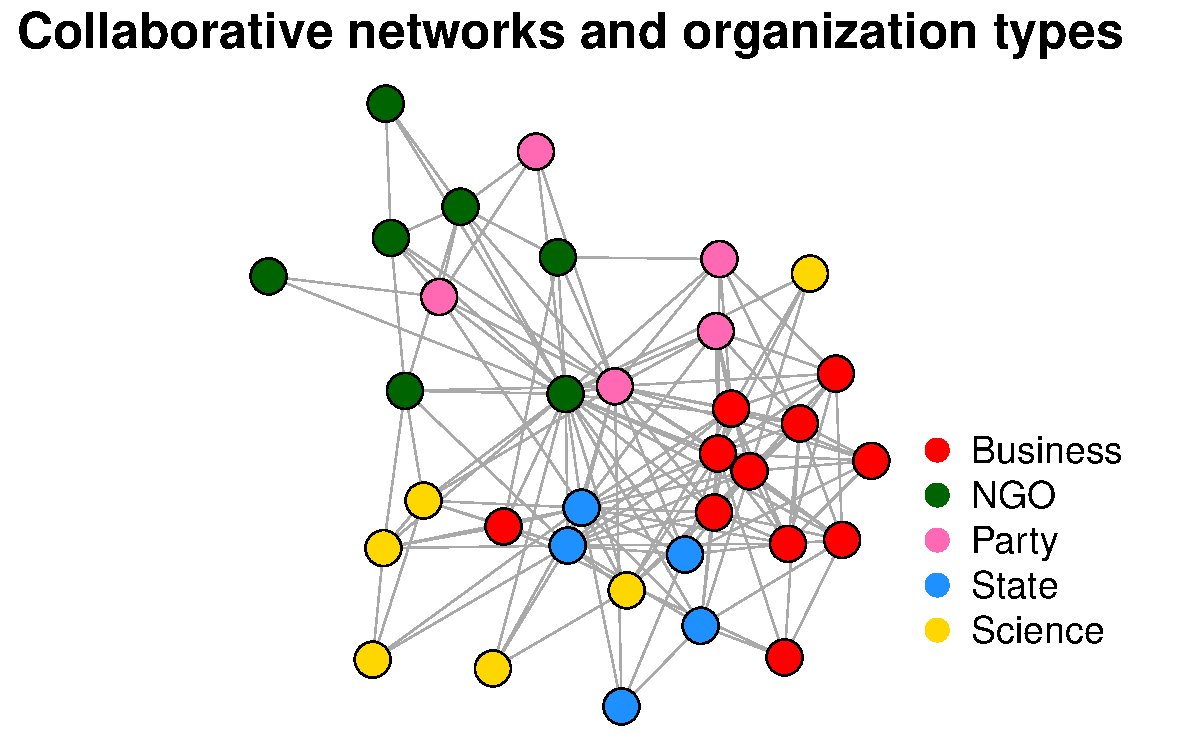
\includegraphics[width=3in]{../Figure/introplot.pdf}	
	\label{fig:intro}
	\caption{You may conjecture that organizations with the same type are more likely to collaborate each other at first glance; but there has been a lack of statistical method to \textbf{test if there exists any significant relationship between network topology and node-specific attributes and if any, which node exerts the most dependency on network.}}
\end{figure}



\subsection*{Introducing two simple Euclidean distance matrix in the context of network}

\begin{figure}[H]
	\centering
	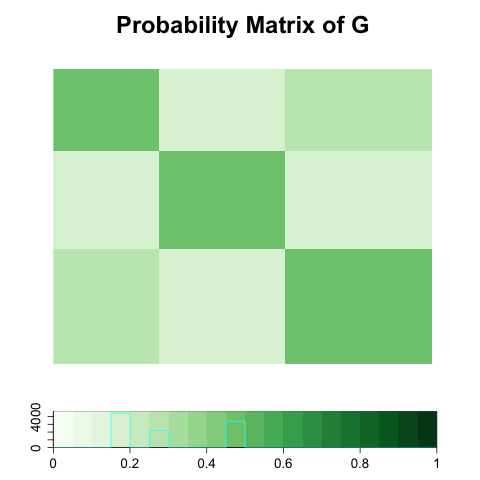
\includegraphics[width=0.23\linewidth]{../Figure/pmat.png} 
	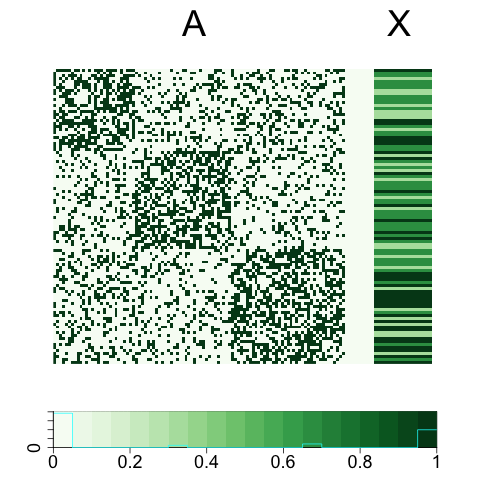
\includegraphics[width=0.23\linewidth]{../Figure/Amat.png}
	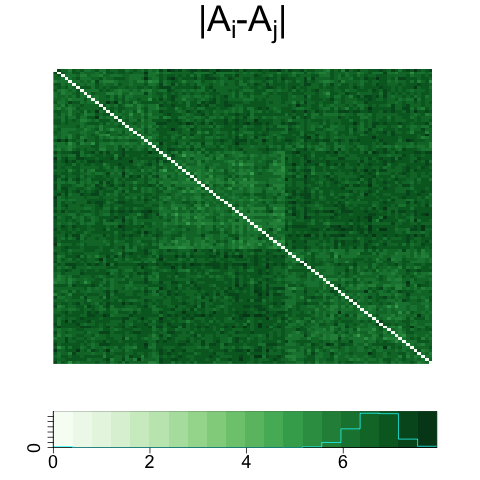
\includegraphics[width=0.23\linewidth]{../Figure/distA.png}
	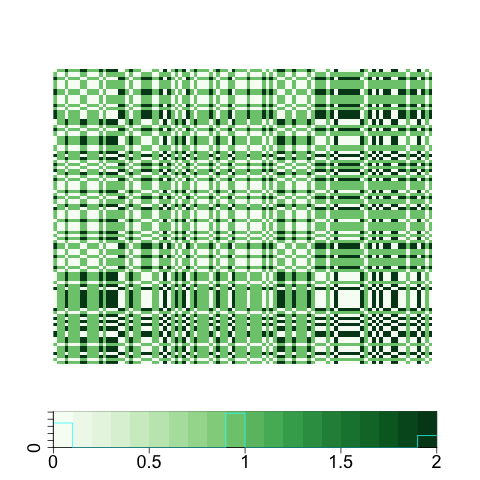
\includegraphics[width=0.23\linewidth]{../Figure/distX.png}
	\caption{Assume that a set of edges follow certain stochastic block model, also depending on the distribution function of nodal attributes $X$ (a), then with some amount of noise we have a realized adjacency matrix and a set of attribute outcomes (b) of which Euclidean distances (c $\&$ d) are suggested to be used in standard distance-based independence test \textbf{but neither of them manifests block structures evident in the data generating model.}}
	\label{fig:matrics}
\end{figure}	

\subsection*{Introduce a family of network distance matrices} 

\begin{figure}[H]
	\centering
	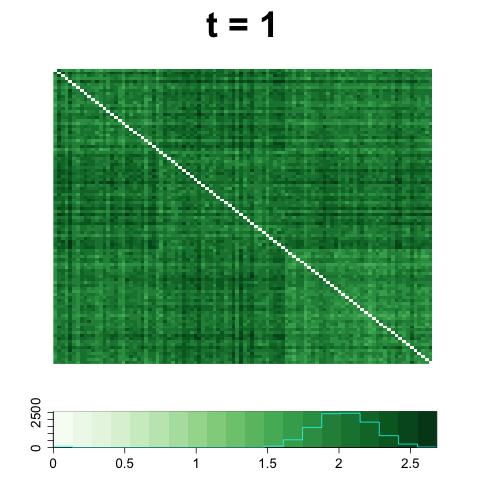
\includegraphics[width=0.3\linewidth]{../Figure/Dx1.png}
	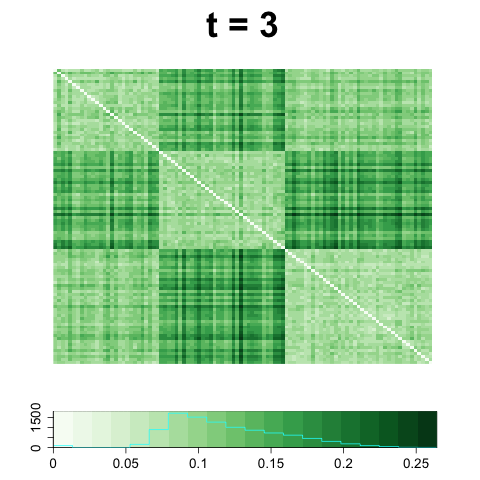
\includegraphics[width=0.3\linewidth]{../Figure/Dx3.png}
	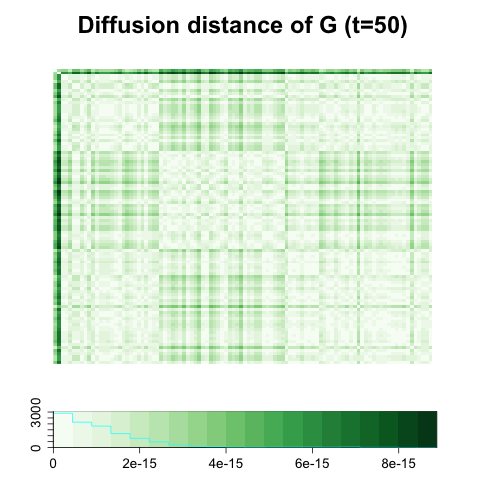
\includegraphics[width=0.3\linewidth]{../Figure/Dx50.png}
	\label{fig:diffusions}
	\caption{\textit{Diffusion matrix}, as a proposed alternative for Euclidean distance of $A$, provides \textbf{one-parameter family of network-based distances} where at early stage, e.g. at $t=1$, distance matrix is very similar to Euclidean distance of $A$ but as time goes by the pattern shown in the distance matrix changes, and \textbf{at optimal time point $t^{*} = 3$ distance matrix shows most clear block structures and at the same time it exhibits most dependence to distance matrix of $\mathbf{X}$.}}
\end{figure}	


\subsection*{ Empirical power of Oracle MGC/Sample MGC}

\begin{figure}[H]
	\centering
	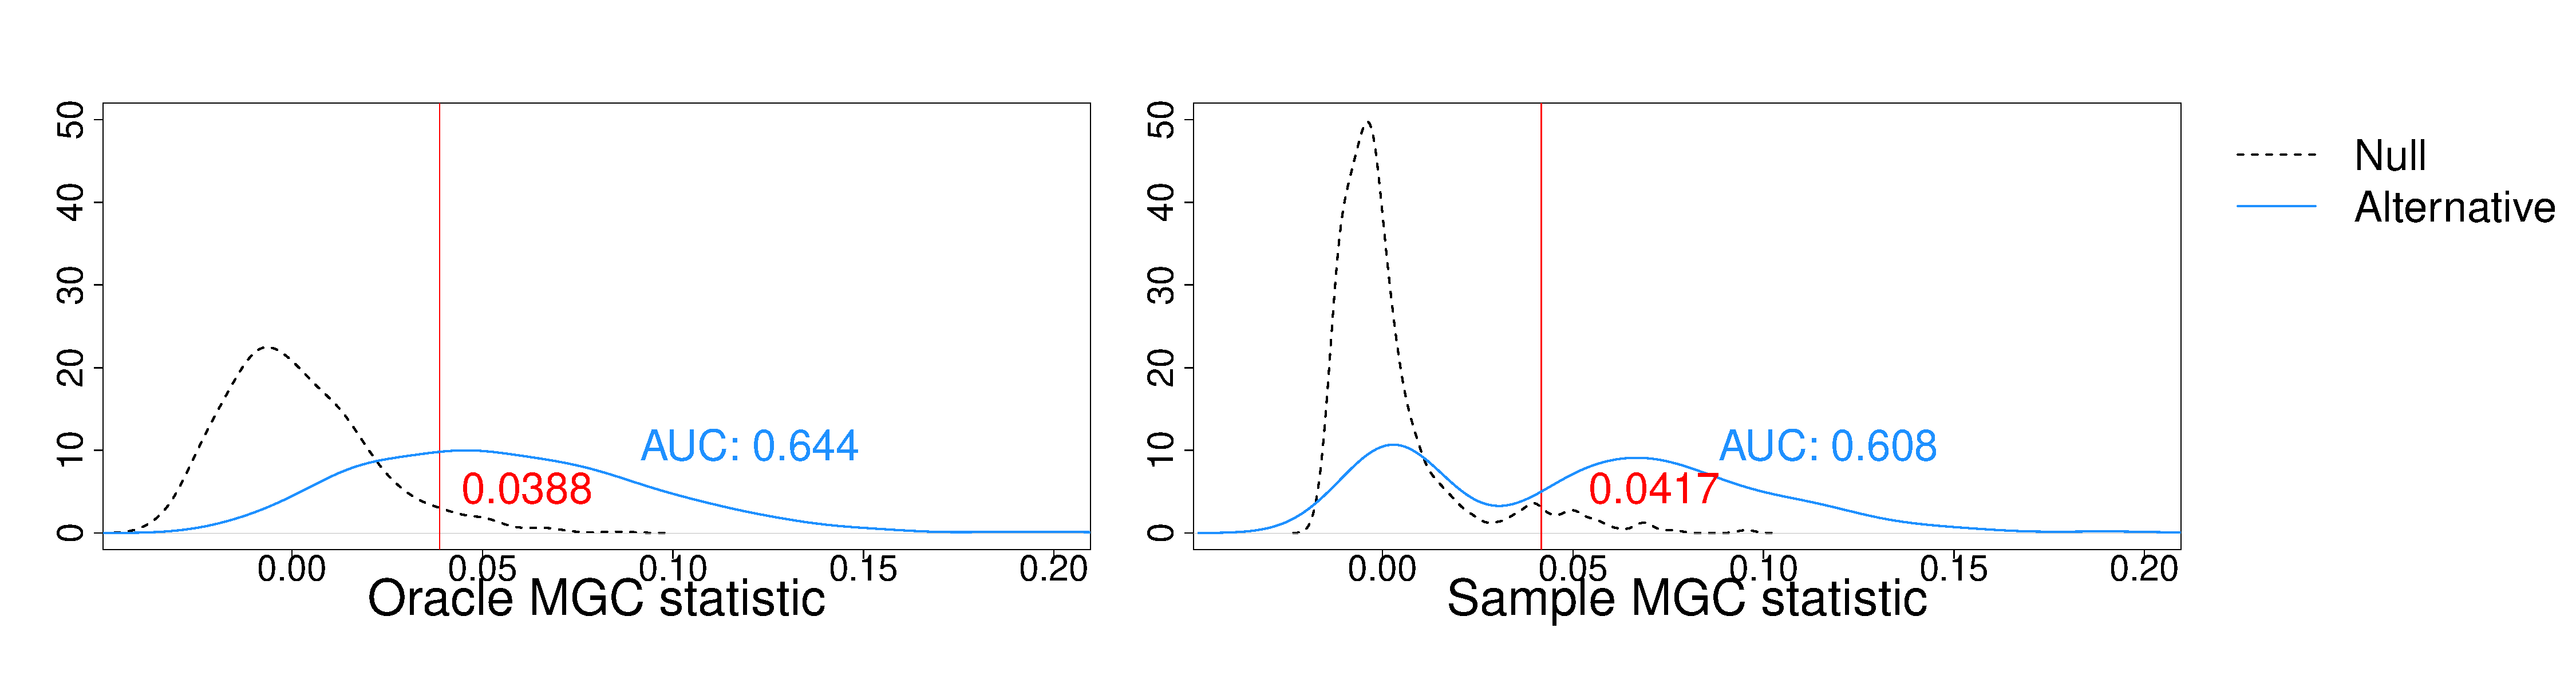
\includegraphics[width=6in]{../Figure/density.pdf}
	\caption{In the left panel we have empirical Null distribution of \texttt{Oracle MGC} illustrated by dotted line of which 95$\%$ sample quantile determines testing power of \texttt{Oracle MGC} by calculating area under the curve (AUC) of the empirical distribution under alternative beyond that quantile, and AUC of \texttt{Oracle MGC} (0.644) looks similar to that of \texttt{Sample MGC} (0.608), as presented in the right panel, even though the shape of its distributions under null and alternative look different, which supports the use of \texttt{Sample MGC} as a substitute for \texttt{Oracle MGC} in real data.}
	\label{fig:density}
\end{figure}	
 
 \newpage
\subsection*{Simplest Stochastic Block Model}
 
\begin{figure}[h]
	\centering
	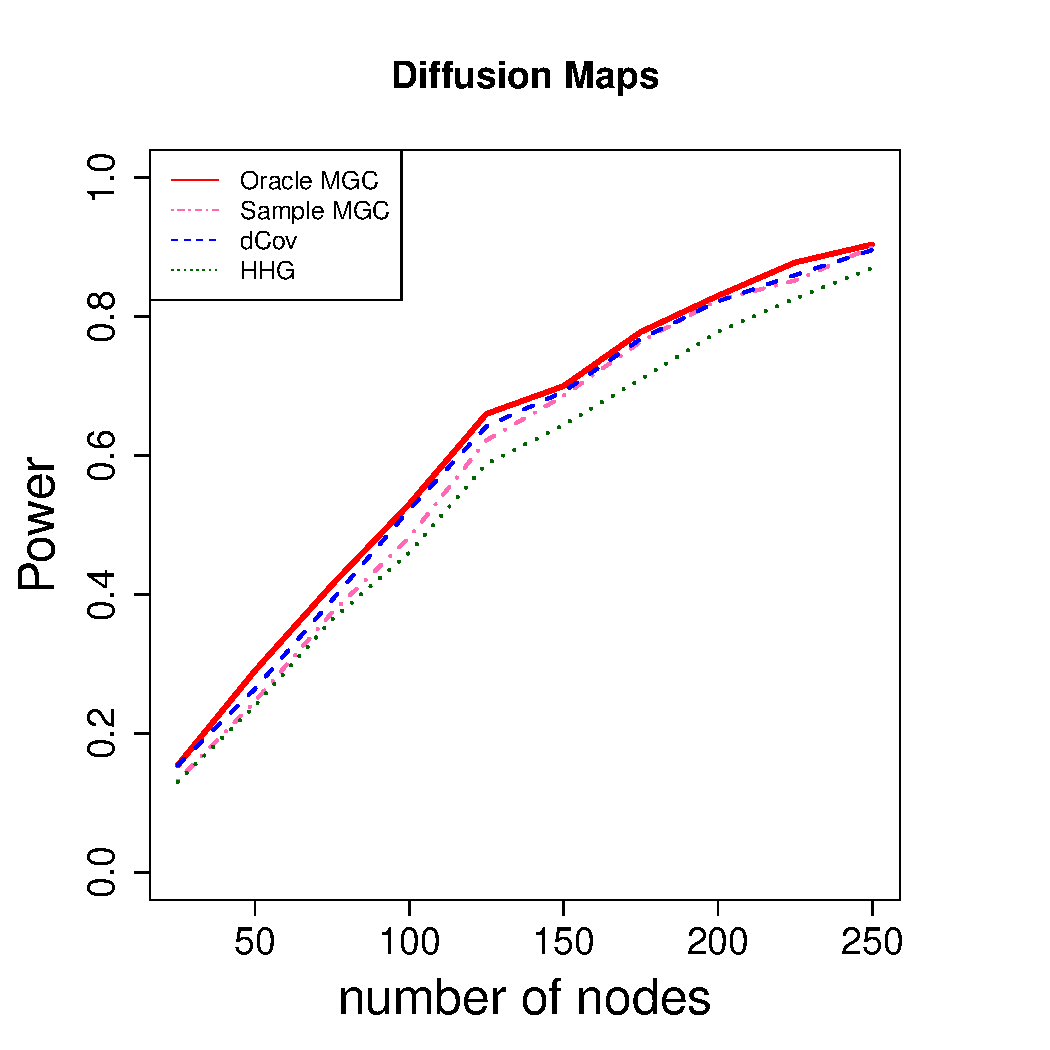
\includegraphics[width=\linewidth]{../Figure/twoSBM.pdf}
	\caption{Above three figures are showing power of three different test statistics under two block SBM using diffusion maps, adjacency matrix, and estimated latent position as a network distance measure, and also \texttt{FH} test results are shown in the left. \textbf{This demonstrates that in the simplest stochastic block model, diffusion distance is generally better than the other two metric; while the performance of \texttt{MGC} statistic is very similar to the others in this case.}}
	\label{fig:twoSBM}
\end{figure}


Alternate : Let \texttt{MGC} = \texttt{Sample MGC}. 

\begin{figure}[h]
	\centering
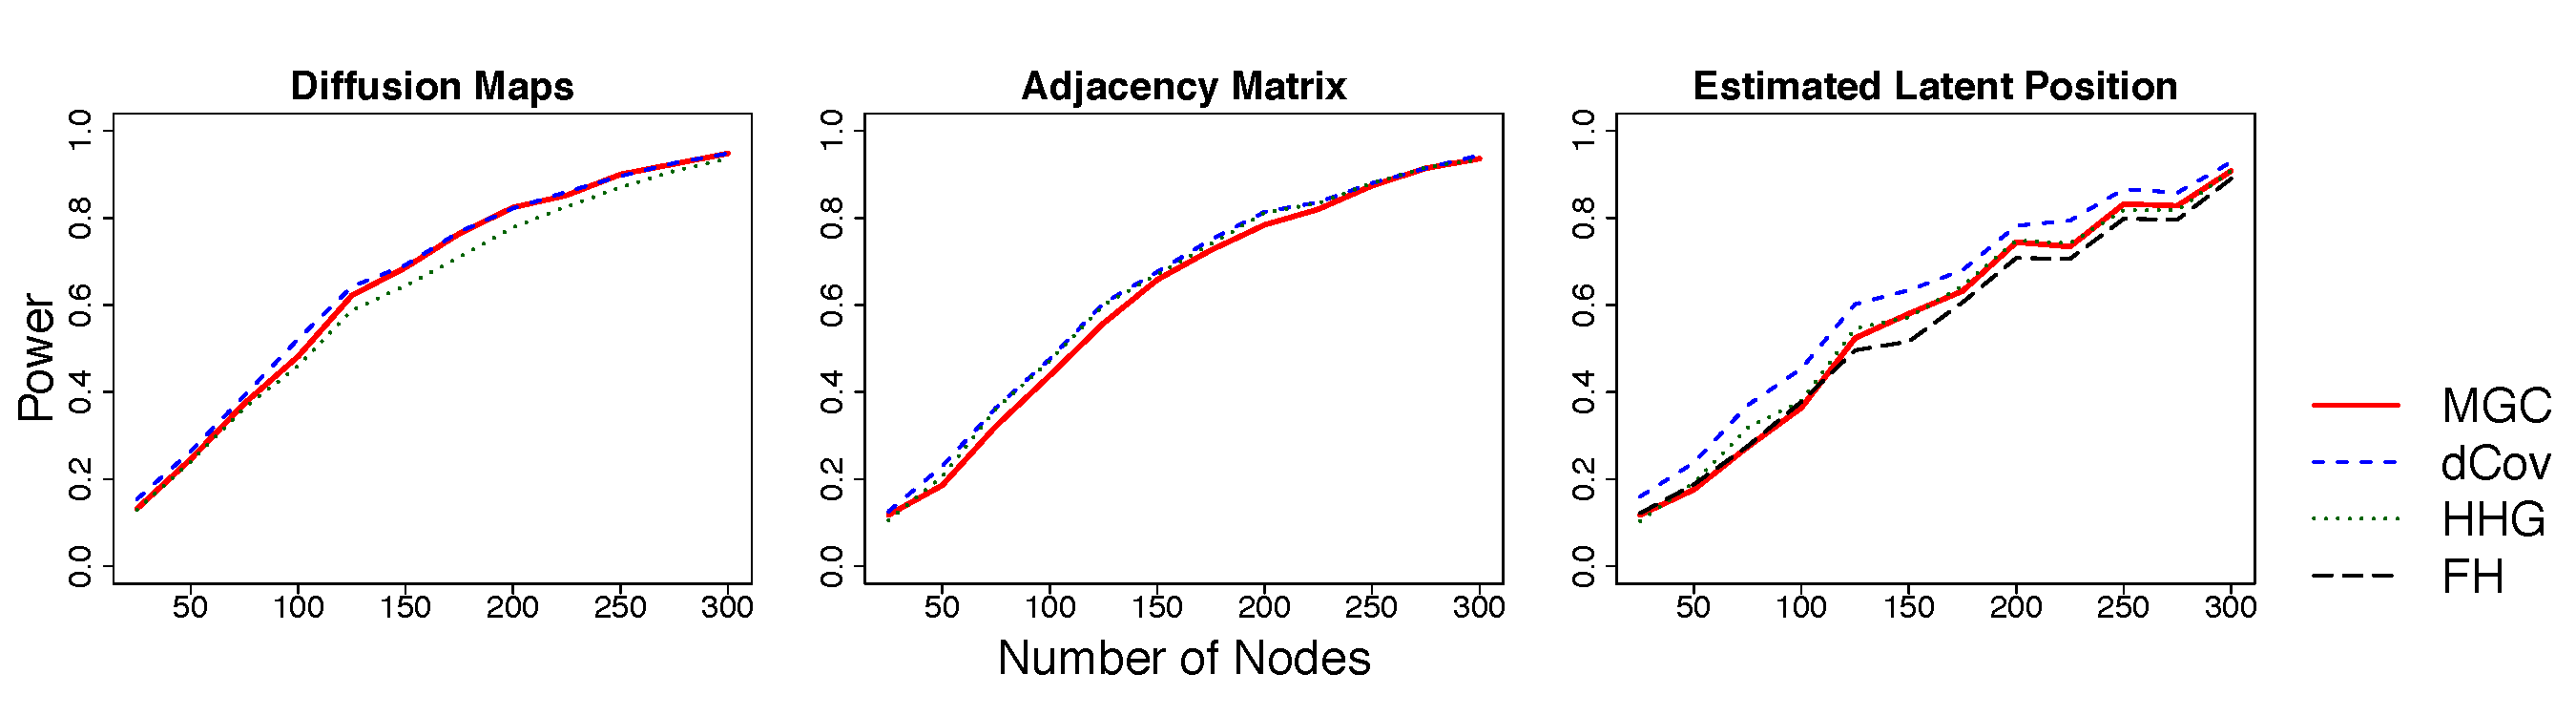
\includegraphics[width=\linewidth]{../Figure/twoSBM_simple.pdf}	
\end{figure}


\newpage
\subsection*{Highest power of MGC under diffusion maps}

\begin{SCfigure}[][h]
	\centering
	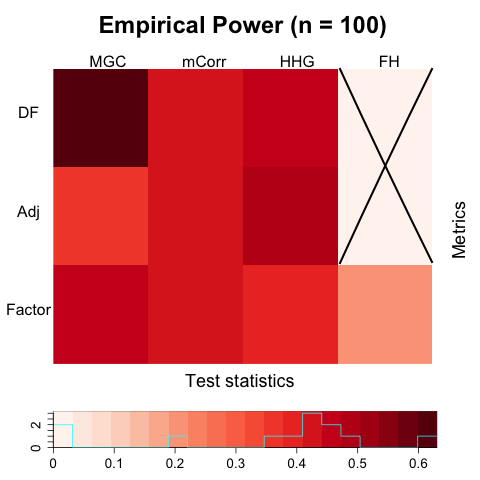
\includegraphics[width=0.38\paperwidth, height=0.33\paperwidth]{../Figure/ThreeSBM_results_simple.png}
	\caption{This power heatmap illustrates the superior power of multiscale generalized correlation (\texttt{MGC}) under diffusion distance matrix (\texttt{DF}) in three SBM (model~\ref{eq:Three}), compared to under adjacency matrix distance (\texttt{Adj}) or latent factor distance (\texttt{Factor}). \textbf{This demonstrates that especially in the presence of nonlinear network dependency, \texttt{MGC} statistic along with a family of diffusion distances catches non monotonic correlations efficiently than the other statistics and metrics.}}
	\label{fig:threeSBM}
\end{SCfigure}


\subsection*{Superiority of the proposed method under non-linear dependency}

\begin{figure}[h]
	\centering
	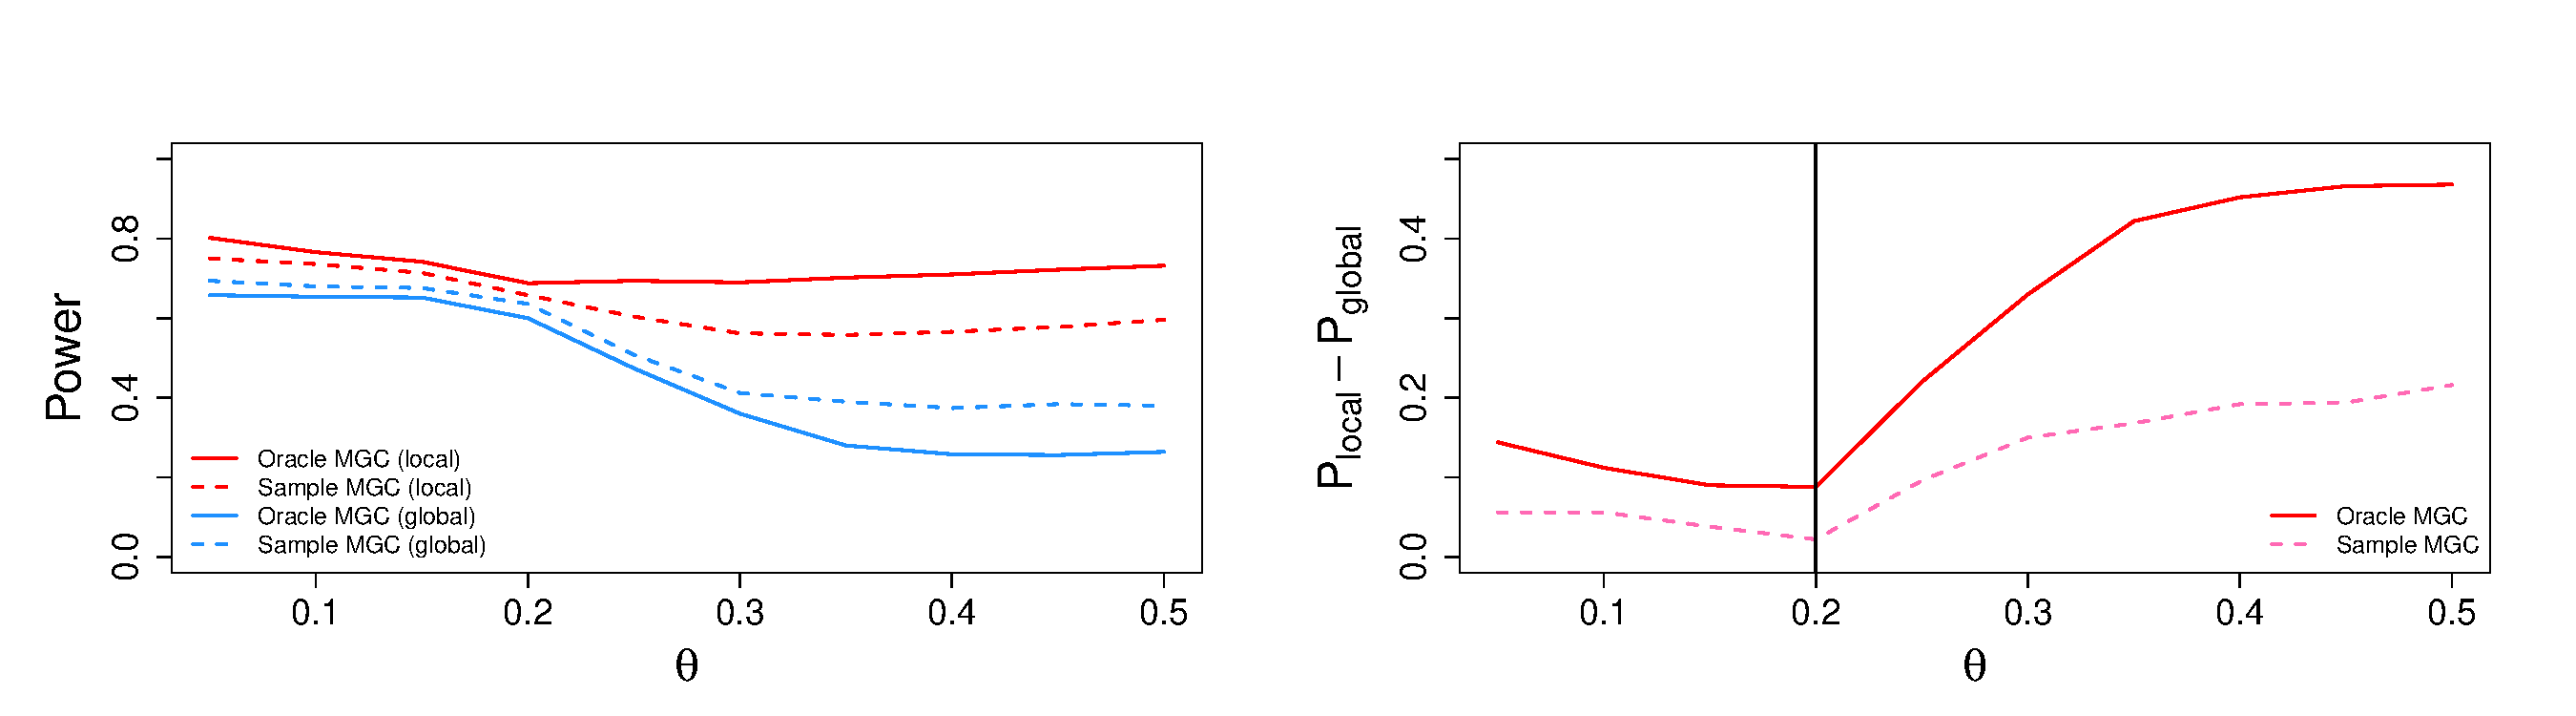
\includegraphics[width=\linewidth]{../Figure/powerplot.pdf}
	\caption{X-axis of $\theta$ controls the existence/amount of nonlinear dependency and in this particular case nonlinearity exists when $\theta > 0.2$ and gets larger as it increases. You can see the discrepancy in power between global and local scale tests also gets larger accordingly, \textbf{mostly due to decreasing power of global test but relatively stable power of \texttt{MGC} under nonlinear dependency} as presented in the left panel.}
	\label{fig:powerplot}
\end{figure}

Alternate : Let \texttt{MGC} = \texttt{Sample MGC}

\begin{figure}[H]
	\centering
	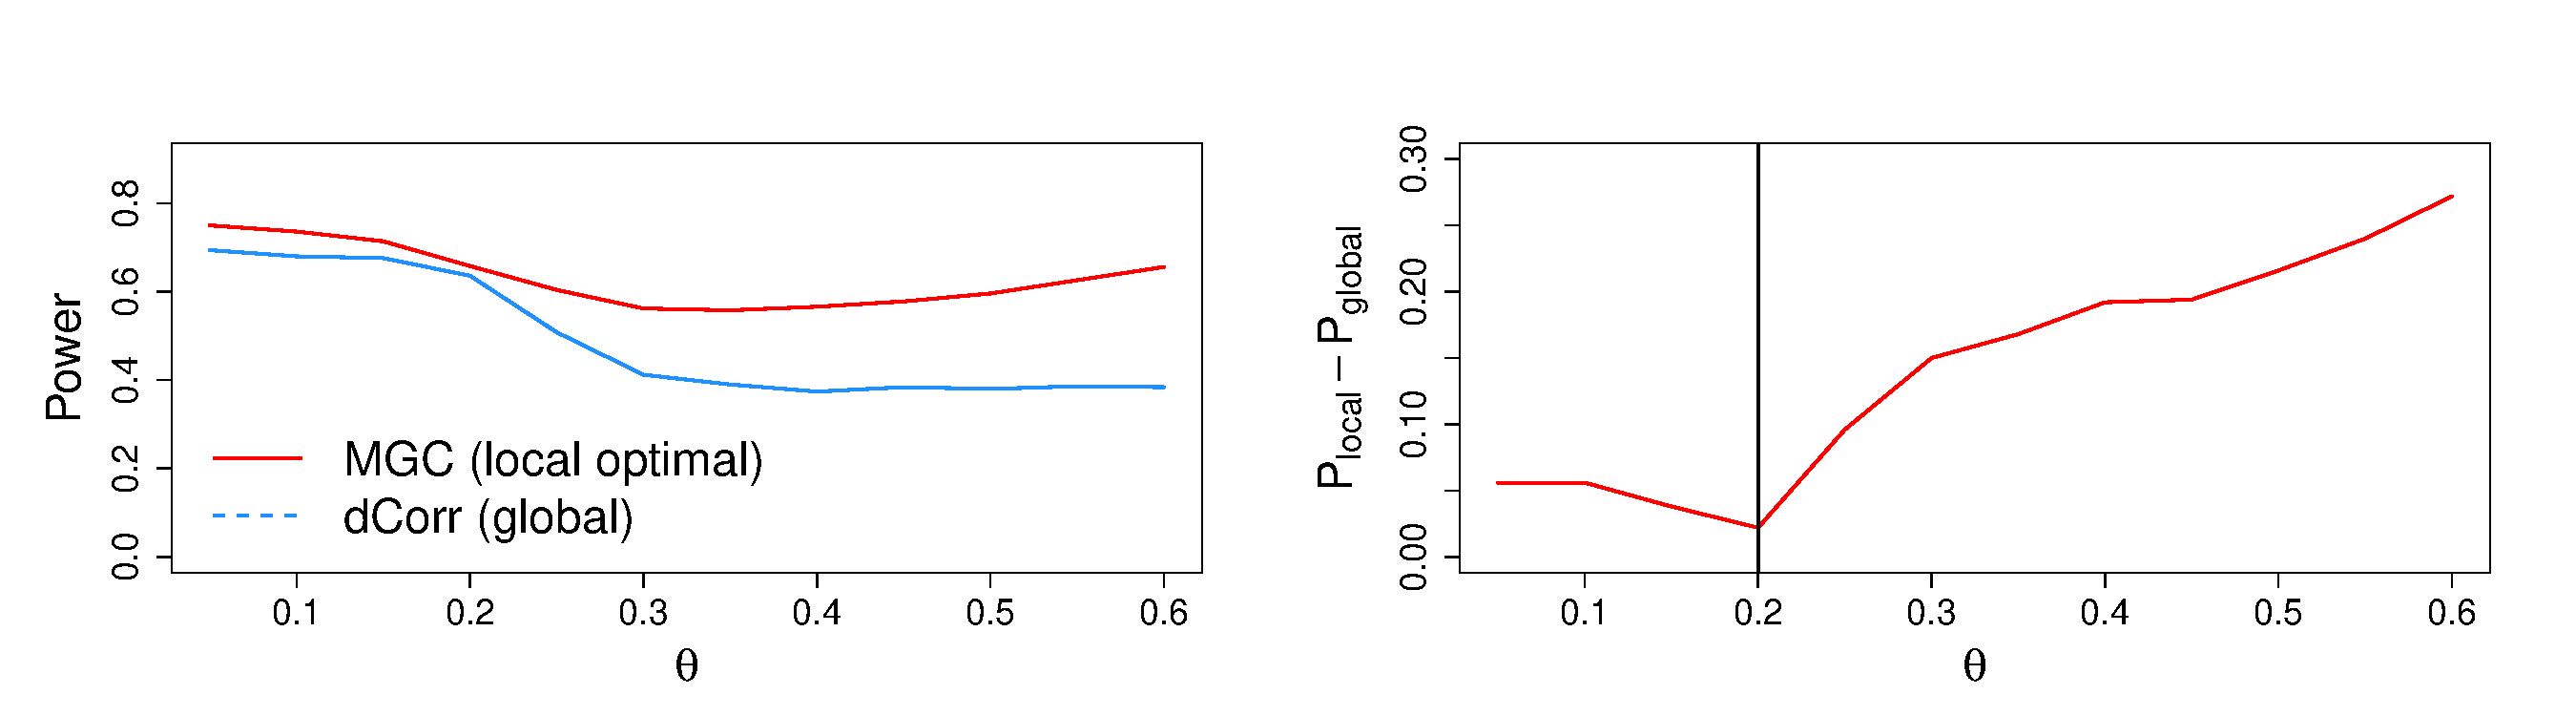
\includegraphics[width=\linewidth]{../Figure/powerplot_simple.pdf}
\end{figure}

\newpage
\subsection*{Degree-corrected SBM with increased variability in node distribution}	

\textbf{Increasing variance in DCSBM}
\begin{equation}
\label{eq:dcVariance}
\begin{gathered}
\begin{aligned}
& \theta_{i} \overset{i.i.d}{\sim} Uniform(1 - \tau, 1 + \tau), i = 1, \ldots, n; \quad \tau = 0, 0.2, \ldots, 1\\ 
& A_{ij} | \mathbf{Z}, \mathbf{\theta}   \overset{i.i.d}{\sim}   f_{A|Z, \theta}(a_{ij} | z_{i}, z_{j}, \theta_{i}, \theta_{j}) \stackrel{d}{=} Bern(0.2 \cdot \theta_{i}\theta_{j}) I ( |z_{i} - z_{j}| = 0 ) \\ & \quad \quad + Bern(0.05 \cdot \theta_{i} \theta_{j} ) I(|z_{i} - z_{j}| = 1), \quad i,j=1, \ldots, n; i < j. 
\end{aligned}
\end{gathered}
\end{equation}


\begin{figure}[h]
	\centering
		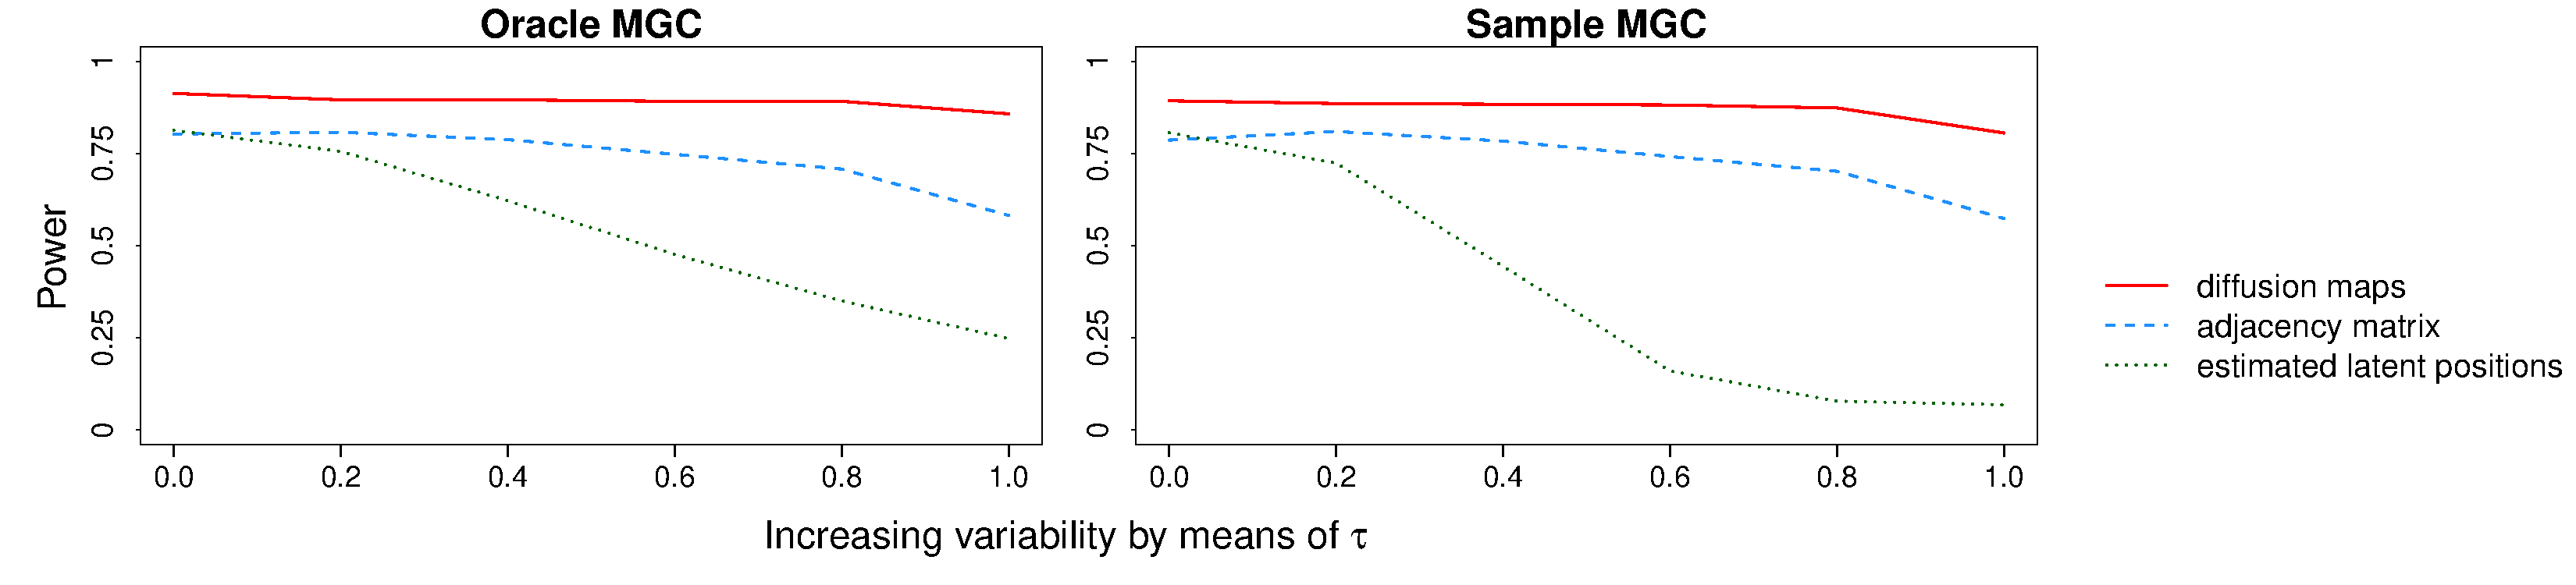
\includegraphics[width=\linewidth]{../Figure/powerplot_var.pdf}
	\caption{In degree-corrected SBM where the variability in degree distribution increases as $\tau$ increases, \textbf{power of diffusion maps are more likely to be robust against increasing variability compared to adjacency matrix and latent positions.}}
	\label{fig:dcSBM}
\end{figure}	

Alternate : Let \texttt{MGC} = \texttt{Sample MGC}

\begin{figure}[H]
	\centering
	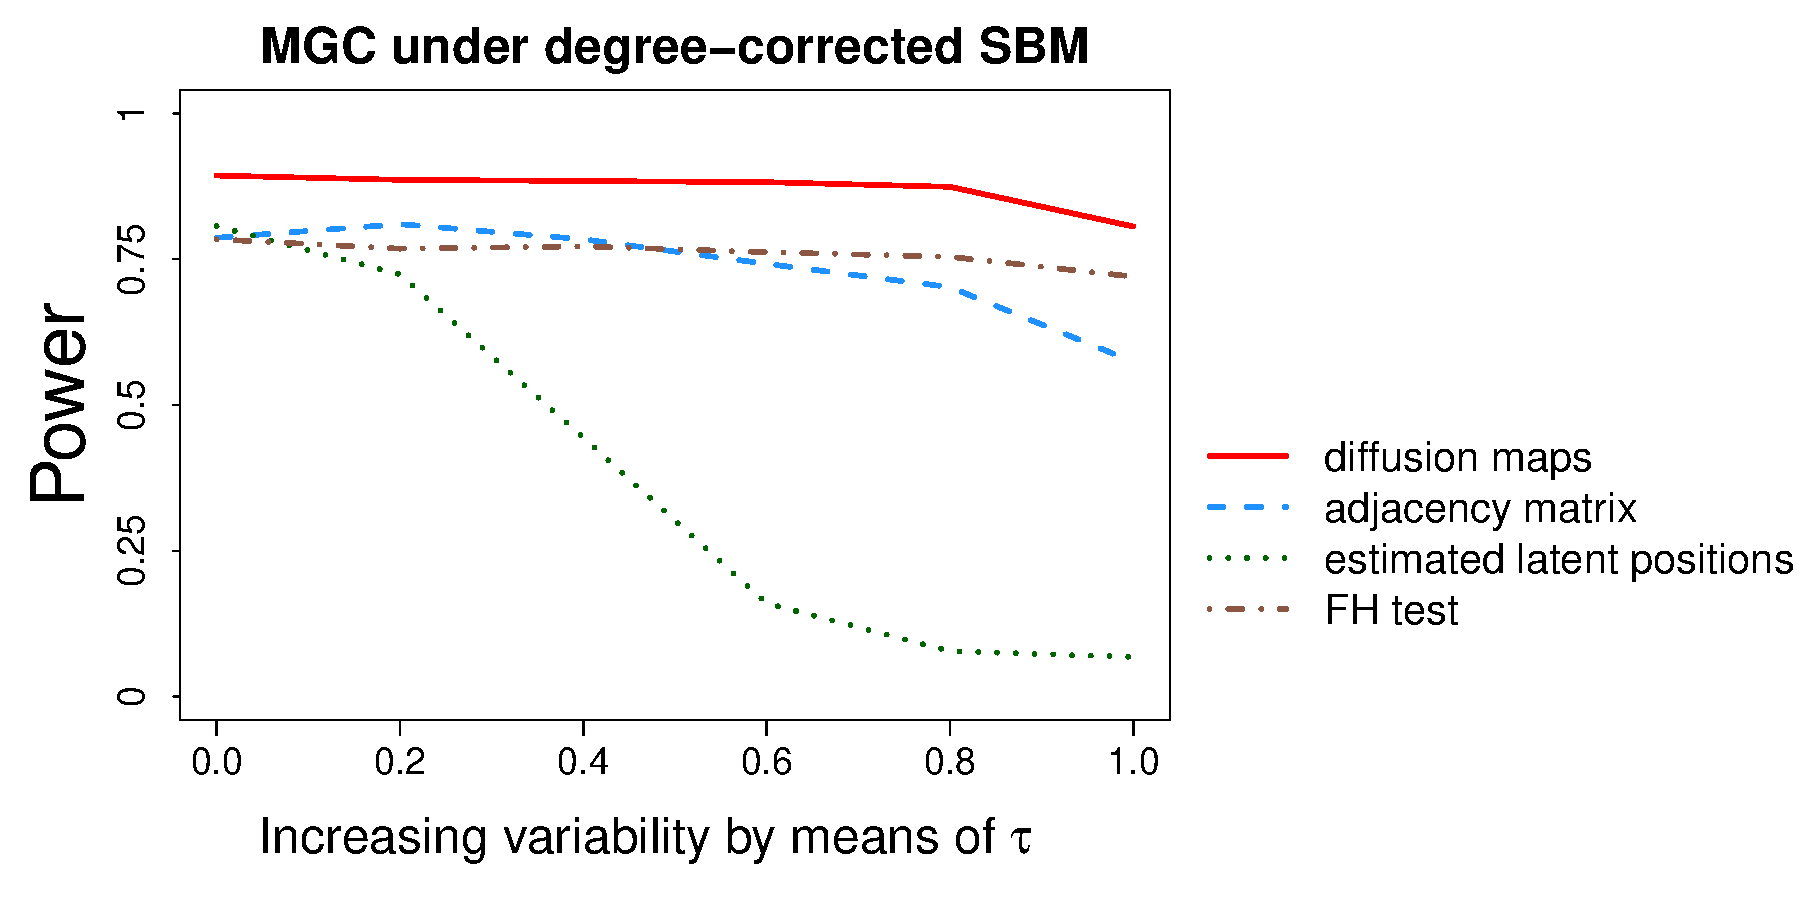
\includegraphics[width=\linewidth]{../Figure/powerplot_var_simple.pdf}
\end{figure}	


\newpage
\subsection*{Validity of the method even under competitor's model}

\begin{figure}[H]
	\centering
	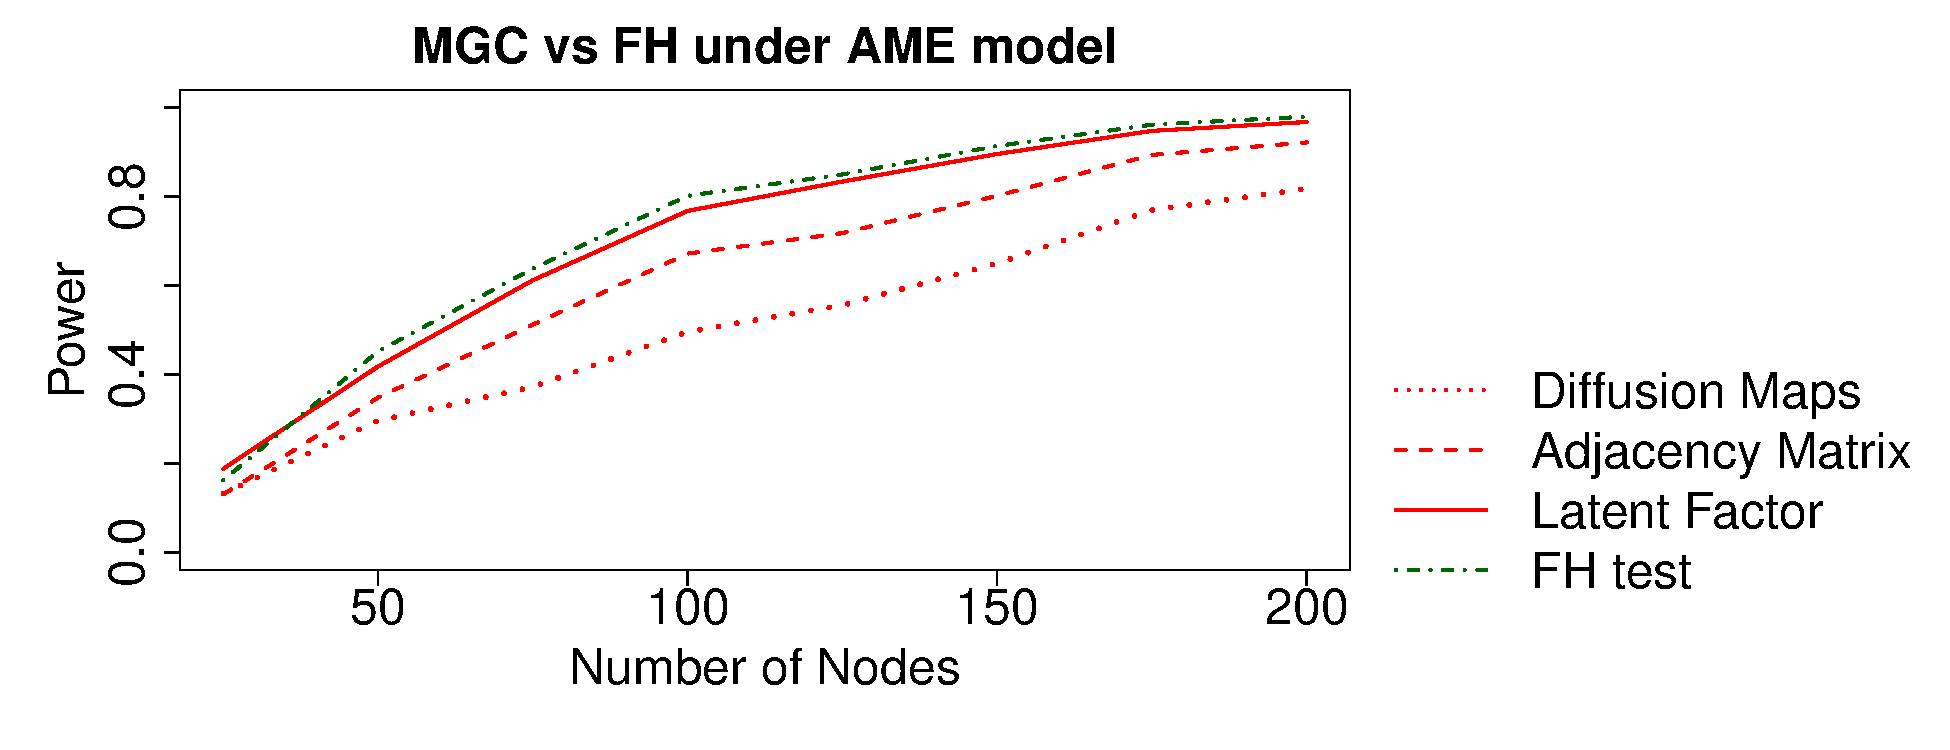
\includegraphics[width=\linewidth]{../Figure/ame_part.pdf}
	\caption{Even under additive and multiplicative model which favors estimated latent position metrics, \texttt{MGC} lost some power when using diffusion maps and adjacency matrix but \textbf{\texttt{MGC} does as good as \texttt{FH} tests under latent factor metrics which is the truth, which supports excellent ability of \texttt{MGC} in diverse, nearly true network metrics.}}
	\label{fig:ame}
\end{figure}	


\subsection*{Node Contribution}

\begin{SCfigure}[][h]
	\centering
		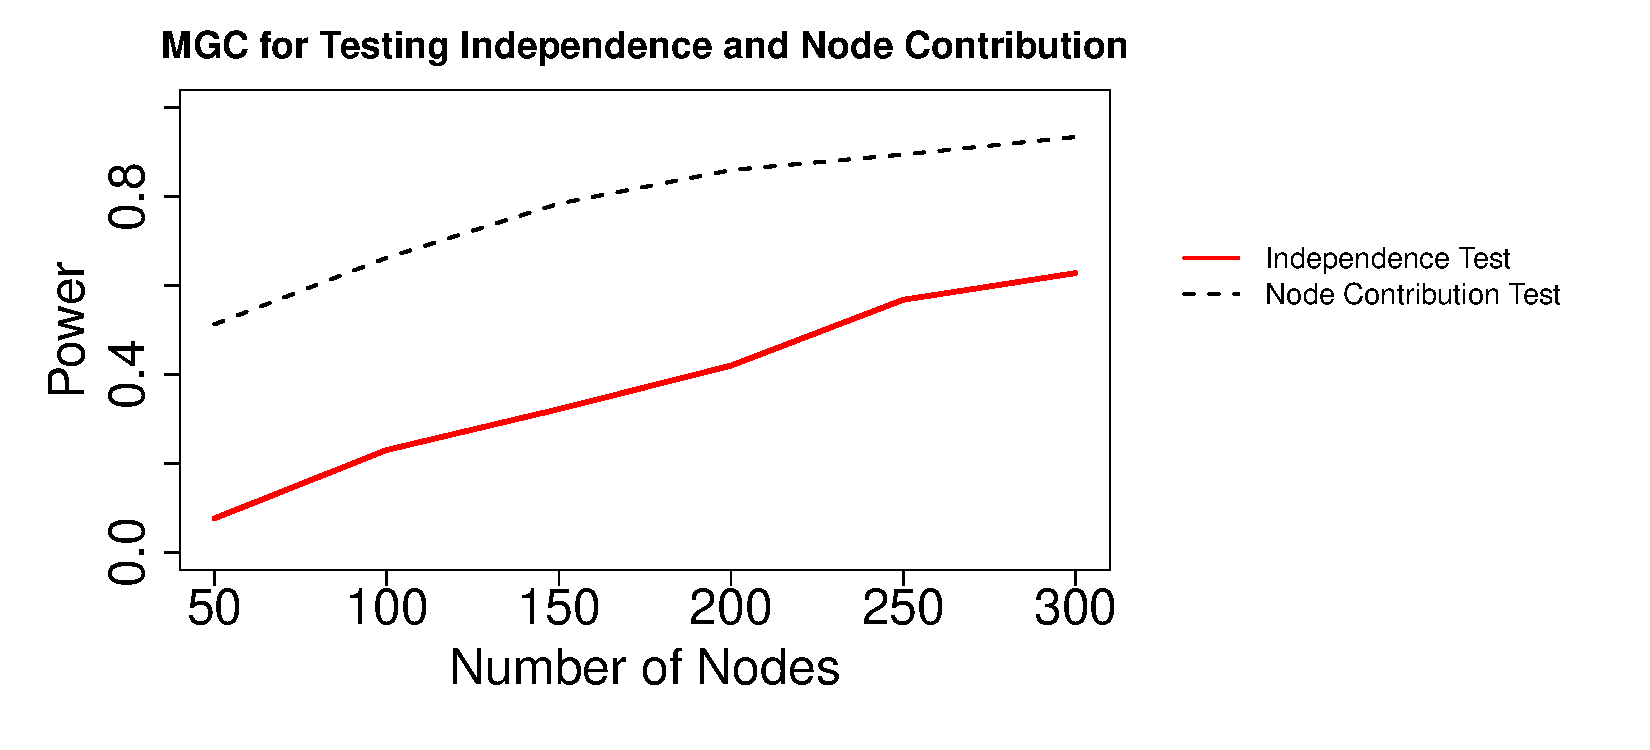
\includegraphics[width=0.6\linewidth, height = 0.3\linewidth]{../Figure/nodecontri.pdf}
	\caption{This plot describes both power of \texttt{MGC} and the rate of correctly-ranked node contribution increase as the number of nodes increases when only half of the nodes for each simulation actually are set to contribute to the independence test, \textbf{which validates the use of node contribution measure in independence test.}}
	\label{fig:contribution}
\end{SCfigure}


\subsection*{Political Network}

\begin{figure}[H]
	\centering
		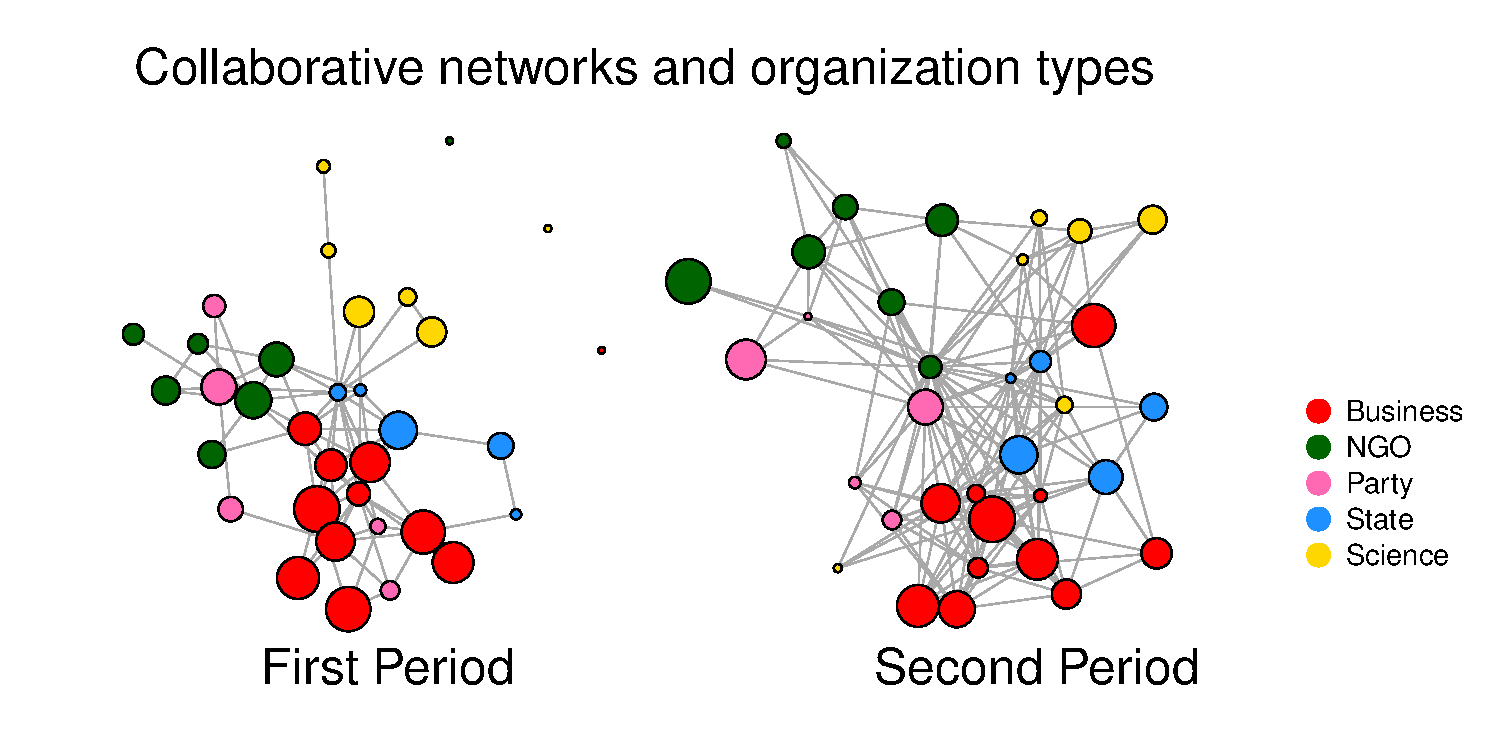
\includegraphics[width=\linewidth]{../Figure/two_politics.pdf}
	\caption{Both networks depict the collaboration network during the two time periods where it turns out significant network dependency in types of organizations. \textbf{Using \texttt{MGC} statistics, we are not only able to test network independence but also rank each node in terms of the amount of contribution to detecting dependence, which is proportional to node size here.}}
	\label{fig:politics}
\end{figure}





\end{document}